% coupling_oil
In this section we consider affecting the light propagation in the second track by changing the surrounding condition. In default condition the experimental setup is placed in vacuum or air. Here the coupling in a different condition is investigated. For the practical experiment there are not many options for changing the environment. In this section the coupling simulation will be placed in an environment full of oil, $n=1.526$ or $\epsilon=2.33$. \\

\begin{figure}[!ht]
\centering
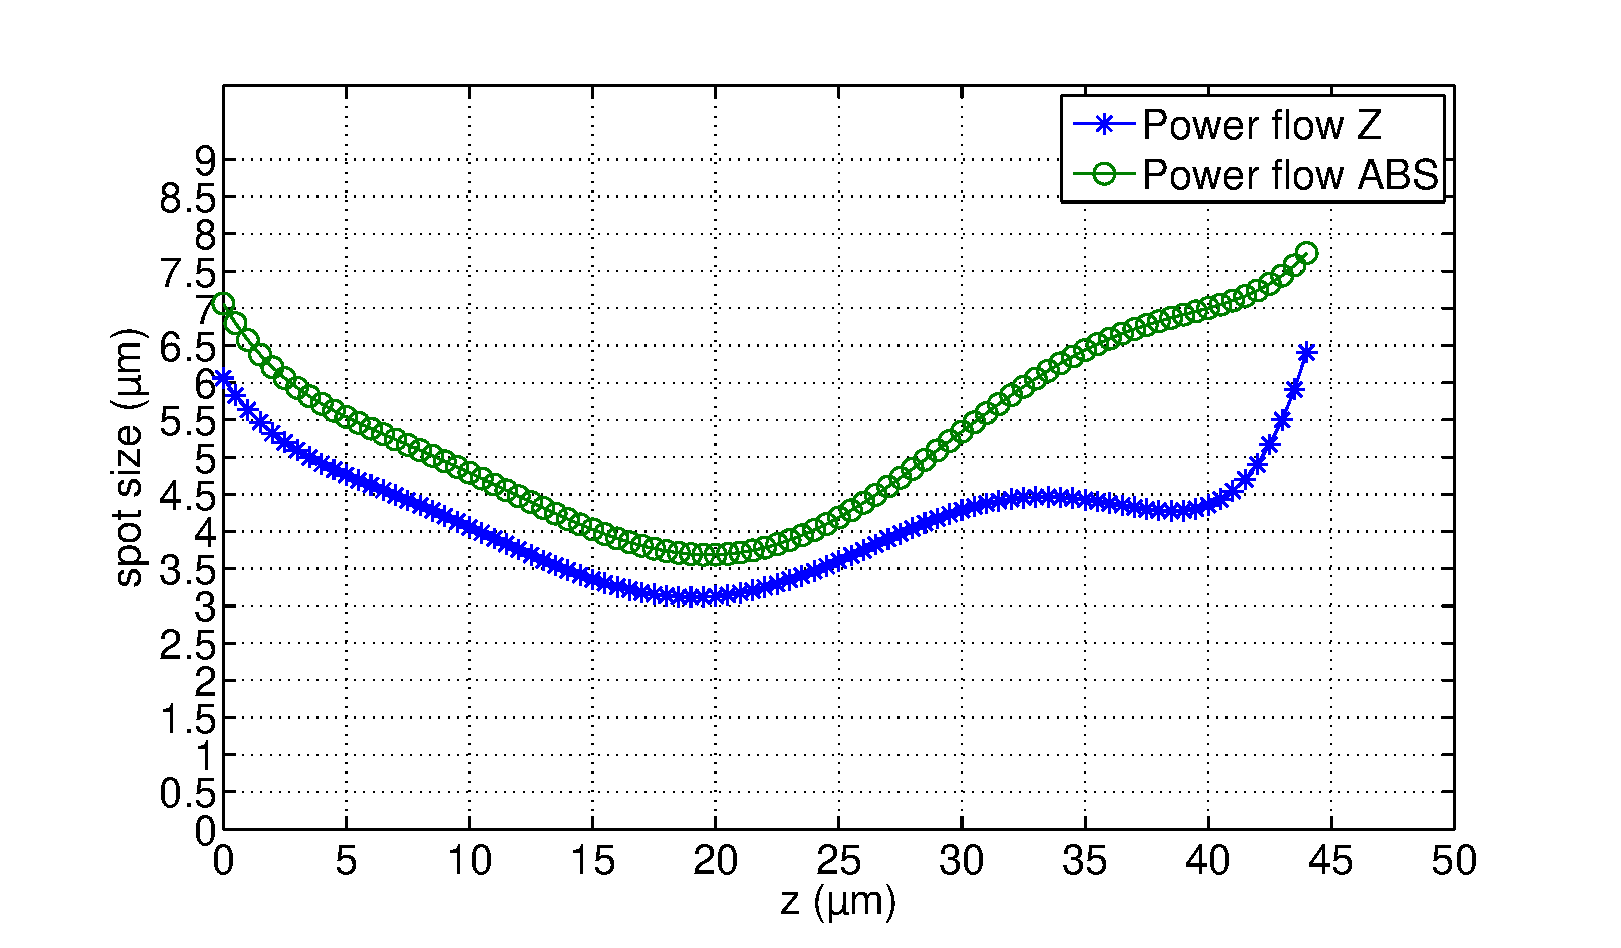
\includegraphics[width=0.7\textwidth]{bilder/spot_curve_oil}
\caption{Spot size curve of TLF in oil. The z-coordinate indicates the distance from TLF end.}
\label{fig:oil_spot_curve}
\end{figure}
Changing around conditions of the simulation may greatly affect the working distance of the TLF. Therefore determining the new working distance is necessary before coupling the TLF to the waveguide.  Similar as in section \ref{sect:model_model_model_TLF} the spot size curve Fig. \ref{fig:oil_spot_curve} can be drawn by loading data of TLF beam propagation in oil from CST MWS. It can be found from that the minimum spot in oil lies at the position of about $19\mu$m from the TLF, farer than the original minimum spot location in air.\\    
\begin{figure}[!ht]
\centering
\includegraphics[width=0.7\textwidth]{bilder/s21_oil_curve}
\caption{Coupling efficiency between TLF and the rib waveguide due to frequency domain in oil background. }
\label{fig:oil_coupling_curve}
\end{figure}

Then in the new coupling setup the waveguide is placed at the new working distance of $19\mu$m. Fig. \ref{fig:oil_coupling_curve} is the $S_{21}$ curve of this arrangement from CST MWS. It shows the coupling efficiency at working frequency $282$THz achieves about $34.5\%$, which is lower than that of the original configuration in section \ref{sect:model_model_model_TLF}. So using oil environment can not improve the coupling ability.\\

